% 128-57(128쪽) — 원문 「오른쪽 그림」. 두 직선 $x=k$, $x=k+1$ 이 곡선 $y=\sqrt{x}$ 및 $x$축과 만나는 점
% $\pt{P}_k$, $\pt{Q}_k$, $\pt{R}_k$, $\pt{S}_k$ 와 색칠한 사각형 $\pt{P}_k\pt{R}_k\pt{S}_k\pt{Q}_k$. 스캔 화질이 낮아 TikZ 로 다시 그림.
% 라벨은 원문 것만 둔다 — $x$, $y$, $\pt{O}$, $\pt{P}_k$, $\pt{Q}_k$, $\pt{R}_k$, $\pt{S}_k$, $k$, $k+1$, $x=k$, $x=k+1$, $y=\sqrt{x}$.
% 눈금을 넣지 않아 $k$ 를 특정 수로 읽을 수 없게 했고, 구하는 합(답)은 그림에 적지 않는다.
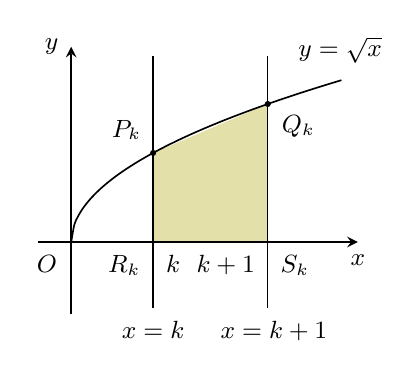
\begin{tikzpicture}[line width=0.6pt, x=0.52cm, y=0.80cm, >=stealth]
  % 사각형 P_k R_k S_k Q_k (윗변은 선분 P_k Q_k)
  \fill[olive!25] (2,0) -- (4.8,0) -- (4.8,2.1909) -- (2,1.4142) -- cycle;
  \draw[->, line width=0.7pt] (-0.8,0) -- (7.0,0) node[below=1pt, font=\small] {$x$};
  \draw[->, line width=0.7pt] (0,-1.15) -- (0,3.10) node[left=1pt, font=\small] {$y$};
  \draw[domain=0:6.60, samples=90, smooth] plot (\x, {sqrt(\x)});
  \draw[line width=0.5pt] (2,-1.05) -- (2,2.95);
  \draw[line width=0.5pt] (4.8,-1.05) -- (4.8,2.95);
  \fill (2,1.4142) circle (2.2pt/2);
  \fill (4.8,2.1909) circle (2.2pt/2);
  \node[anchor=north east, font=\small] at (-0.1,-0.05) {$\pt{O}$};
  \node[anchor=south east, font=\small] at (1.95,1.46) {$\pt{P}_k$};
  \node[anchor=north west, font=\small] at (4.90,2.17) {$\pt{Q}_k$};
  \node[anchor=north east, font=\small] at (1.93,-0.05) {$\pt{R}_k$};
  \node[anchor=north west, font=\small] at (2.07,-0.05) {$k$};
  \node[anchor=north east, font=\small] at (4.73,-0.05) {$k+1$};
  \node[anchor=north west, font=\small] at (4.87,-0.05) {$\pt{S}_k$};
  \node[anchor=west, font=\small] at (5.30,3.05) {$y=\sqrt{x}$};
  \node[anchor=north, font=\small] at (2,-1.10) {$x=k$};
  \node[anchor=north, font=\small] at (4.95,-1.10) {$x=k+1$};
\end{tikzpicture}
